\documentclass[letterpaper]{article}
\usepackage[utf8]{inputenc}
\usepackage[spanish]{babel}
\usepackage{amssymb, amsmath}
\usepackage{stackengine}
\usepackage{graphicx}
\usepackage{lipsum}
\usepackage{dsfont}
\usepackage[margin=1.5cm,
vmargin={1.5cm,0.7cm},
includefoot]{geometry}
\usepackage{setspace}
\usepackage{subcaption}
\usepackage{tocloft}
\usepackage{upgreek}
\usepackage{amsthm}
\usepackage{graphicx}
\usepackage{paralist}
\usepackage{fancyhdr}
\usepackage{lmodern}
\usepackage{tcolorbox}
\usepackage{color}
\usepackage{tikz}
\usepackage{wasysym}
\usepackage{textgreek, marvosym}
\tcbuselibrary{skins,breakable}
\pagestyle{fancy}

\renewcommand{\headrulewidth}{0.4pt}
\renewcommand{\footrulewidth}{0.4pt}

\renewcommand{\d}{\partial}

\providecommand{\abs}[1]{\left|#1\right|}
\providecommand{\norm}[1]{\left|\left|#1\right|\right|}														  
\providecommand{\pint}[1]{\langle#1\rangle}														  
\newcommand{\V}{\mathds{V}}

\newcommand{\W}{\mathds{W}}

\newcommand{\F}{\mathds{F}}

\newcommand{\tq}{ \quad \cdot  \backepsilon \cdot \quad }

\newcommand{\ld}{\lim\limits_{x \to 0^{+}}}

\newcommand{\li}{\lim\limits_{x \to 0^{-}}}

\newcommand{\la}{\lim\limits_{x \to a}}

\renewcommand{\l}{\ell}

\newcommand{\R}{\mathds{R}}

\newcommand{\Po}{\mathds{P}_2(\mathds{R})}

\renewcommand{\*}{\cdot}

\newcommand{\Iden}{\begin{pmatrix}
		1 & 0 & 0\\
		0 & 1 & 0\\
		0 & 0 & 1 
\end{pmatrix}}
\newcommand{\T}{\begin{pmatrix}
		1 & 3 & 9 \\
		1 & 3 & 4 \\
		0 & 0 & 2 
\end{pmatrix} }

\makeatletter
\renewcommand*\env@matrix[1][\arraystretch]{%
	\edef\arraystretch{#1}%
	\hskip -\arraycolsep
	\let\@ifnextchar\new@ifnextchar
	\array{*\c@MaxMatrixCols c}}
\makeatother

\newtheorem{theorem}{Teorema}[section]
\theoremstyle{definition}
\newtheorem{definition}{Definición}


\begin{document}
	
	\setlength{\unitlength}{1cm}
	\thispagestyle{empty}
	\begin{picture}(19,3)
	\put(-0.5,1.2){
\includegraphics[scale=.20]{img/unam1.png}}
	\put(16,1){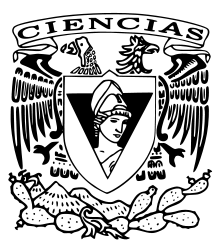
\includegraphics[scale=.29]{img/fciencias1.png}}
	\end{picture}
	
	\begin{center}
		\vspace{-114pt}
		\textbf{\large Matemáticas para las Ciencias II}\\
		\textbf{ Semestre 2020-2}\\
		Prof. Pedro Porras Flores\\
		Ayud. Irving Hernández Rosas \\
		\textbf{Proyecto V}\\[0.2cm]
		Kevin Ariel Merino Peña\footnote{Número de cuenta 317031326}\\ [0.2cm]
	\end{center}
	\vspace{-10pt}
	\rule{19cm}{0.3mm}
	
\noindent Realice los siguientes ejercicios, escribiendo el procedimiento claramente. Y recuerden que estos proyectos se entregan de manera individual en la plataforma de google classroom.\\

% -----------------------------------------------------
% Problema uno
% -----------------------------------------------------
\noindent1.  Verifique el primer caso de la regla de la cadena de la composición $ f\circ \vec{\gamma}$ para cada uno de los siguientes casos, esto es primero haga la composición y derive, y le luego use la regla de la cadena y vea que se llega al mismo resultado.\\


a) $f(x,y) = xy$, $\vec{\gamma}(t) =(e^t, \cos(t)) $.\\

b) $f(x,y) = xy$, $\vec{\gamma}(t) =(3t^2, t^3) $.\\

c) $f(x,y) = (x^2 + y^2)\ln{\sqrt{x^2 + y^2}}$, $\vec{\gamma}(t) =(e^t, e^{-t}) $.\\

d) $f(x,y) = xe^{x^2 + y^2}$, $\vec{\gamma}(t) =(t, -t) $.\\





\noindent2. Sea $f(u, v, w) = (e^{u -w}, \cos{(u + v)} + \sin{(u + v + w)})$ y $g(x,y) = (e^{x}, \cos{(y - x)}, e^{-y} )$. Calcule $ f\circ g$ y $\mathbf{D}(f\circ g)(0,0)$.\\

\noindent3.  Calcule la derivada direccional de las siguientes funciones en el punto y la dirección dada: \\


a) $f(x,y) = x + 2xy -3y^2$, $(x_0, y_0) = (1,2)$ y $\vec{v} = \frac{3}{5}\hat{e}_1 + \frac{4}{5}\hat{e}_2 $.\\

b) $f(x,y) = \ln{\sqrt{x^2 + y^2}}$, $(x_0, y_0) = (1,0)$ y $\vec{v} = \left( \frac{1}{\sqrt{5}} \right)(2\hat{e}_1 + \hat{e}_2 )$.\\

c) $f(x,y) = e^x\cos{(\pi y)}$, $(x_0, y_0) = (0,-1)$ y $\vec{v} = - \left( \frac{1}{\sqrt{5}} \right)\hat{e}_1 +  \left( \frac{2}{\sqrt{5}} \right)\hat{e}_2 $.\\

d) $f(x,y) = xy^2 + x^3y$, $(x_0, y_0) = (4,-2)$ y $\vec{v} =  \left( \frac{1}{\sqrt{10}} \right)\hat{e}_1 +  \left( \frac{3}{\sqrt{10}} \right)\hat{e}_2 $.\\


\noindent4. Encuentre un vector que sea normal a la curva $x^3 + xy + y^3 = 11$ en  $(1,2)$.\\

\noindent5.  El Capitán Ralphis se encuentra en problemas cerca del lado soleado de Mercurio. La temperatura del casco del barco cuando está en la ubicación $(x, y, z)$ estará dada por $T(x,y,z) = e^{-x^2 - 2y^2 - 3z^2}$, donde $x,y,z$ se miden en metros. Actualmente está en $(1,1,1)$.\\

a) ¿En qué direcciones debería proceder para disminuir la temperatura más rápidamente?\\

b) Si el barco viaja a $e^8$ metros por segundo, ¿qué tan rápido será la disminución de la temperatura si avanza en esa dirección?\\

c) Desafortunadamente, el metal del casco se romperá si se enfría a una velocidad superior a $\sqrt{14}e^2$ grados por segundo. Describa el conjunto de posibles direcciones en las que puede proceder a bajar la temperatura a no más de esa tasa.\\






\end{document}
